% !TEX program = xelatex
% 本文件为第二章独立解答。建议用 XeLaTeX 编译两次。
\documentclass[UTF8,a4paper,11pt]{ctexart}
\usepackage[a4paper,margin=2.15cm,headheight=16pt]{geometry}
\usepackage{amsmath,amssymb,mathtools,bm}
\usepackage{booktabs,longtable,array,enumitem}
\usepackage[most]{tcolorbox}
\usepackage{tikz}
\usepackage{xcolor,fancyhdr,hyperref}
\usepackage{microtype}
\definecolor{navy}{HTML}{264B86}
\definecolor{blue}{HTML}{356BA8}
\definecolor{pink}{HTML}{B84F82}
\definecolor{palepink}{HTML}{FBEAF2}
\definecolor{pale}{HTML}{EAF3FB}
\definecolor{gray}{HTML}{536171}
\hypersetup{colorlinks=true,linkcolor=navy,urlcolor=blue,pdftitle={常微分方程（第三版）第二章习题详细解答}}
\setlength{\parindent}{2em}
\setlength{\parskip}{0.28em}
\setlist[enumerate]{leftmargin=2.2em,itemsep=0.45em,topsep=0.35em}
\pagestyle{fancy}
\fancyhf{}
\fancyhead[L]{\small\color{gray}《常微分方程》（第三版）习题解答}
\fancyhead[R]{\small\color{pink}第二章·基本定理}
\fancyfoot[C]{\small\thepage}
\renewcommand{\headrulewidth}{0.4pt}
\newcommand{\dd}{\,\mathrm d}
\newcommand{\e}{\mathrm e}
\newcommand{\R}{\mathbb R}
\newcommand{\note}[1]{\par\smallskip\noindent\textcolor{pink}{\bfseries 说明：}#1\par\smallskip}
\tcbset{
  exercisebox/.style={enhanced,breakable,arc=0pt,outer arc=0pt,
    boxsep=0pt,left=10pt,right=10pt,top=10pt,bottom=10pt,
    before skip=10pt,after skip=6pt,
    coltitle=navy,fonttitle=\bfseries,toptitle=6pt,bottomtitle=6pt,
    titlerule=0.4pt}
}
\newtcolorbox{problem}[1]{exercisebox,
  colback=white,colframe=blue,colbacktitle=pale,
  boxrule=0.55pt,leftrule=2pt,
  title={题目\quad #1}}
\newtcolorbox{solution}{exercisebox,
  colback=palepink!15!white,colframe=pink,colbacktitle=palepink,
  boxrule=0.45pt,leftrule=2pt,
  title={解答}}
\newtcolorbox{analysis}{exercisebox,
  colback=pale!30!white,colframe=blue,colbacktitle=pale,
  boxrule=0.4pt,leftrule=2pt,
  title={分析}}
\newcommand{\sect}[1]{\section*{\textcolor{navy}{习题 #1}}}

\begin{document}
\begin{center}
  {\LARGE\bfseries\color{navy}常微分方程（第三版）第二章习题解答\par}
  \vspace{0.35em}
  {\color{pink}基本定理 · 习题 2.1--2.5\par}
\end{center}
\begin{center}
  \small\color{gray}本答案使用 AI 工具制作，请读者确认正确性后再使用。除非题目另有说明，本稿接受隐式解。
\end{center}
\sect{2.1}
\begin{problem}{2.1-1}
试绘出下列方程的积分曲线：
  \begin{enumerate}[label=(\arabic*)]
    \item $y'=a$（$a$ 为常数）；
    \item $y'=x^2$；
    \item $y'=|y|$；
    \item $\displaystyle \frac{dy}{dx}=\frac{1}{x^2}$；
    \item $\displaystyle \frac{dy}{dx}=|x|$。
  \end{enumerate}
\end{problem}

\begin{solution}
\begin{enumerate}[label=(\arabic*)]
\item 积分得 $y=ax+C$，所以积分曲线是一族斜率均为 $a$ 的平行直线；$a=0$ 时为水平直线。
\item 积分得 $y=x^3/3+C$。各曲线互为竖直平移，因 $y'=x^2\ge0$ 而处处不下降，在 $x=0$ 有水平切线。
\item $y=0$ 是一条积分曲线。初值为正时 $y'=y$，得 $y=Ce^x$（$C>0$）；初值为负时 $y'=-y$，得 $y=-Ce^{-x}$（$C>0$）。这两族曲线都在横轴的一侧，且不能与零解相交。前者向右上升，后者向右上升并趋近横轴。
\item 在 $x\ne0$ 的每个连通区间内，$y=-1/x+C$。$x=0$ 处方程无定义，左右两侧的曲线不能合为经过 $x=0$ 的解。
\item 分别在 $x\ge0$、$x\le0$ 积分，并令曲线在 $x=0$ 连续，得
\[
y=\frac12x|x|+C=
\begin{cases}C+x^2/2,&x\ge0,\\C-x^2/2,&x\le0.\end{cases}
\]
每条曲线在原点所在的竖线上有水平切线，向左、向右都单调上升。
\end{enumerate}
作图时分别画出上述曲线的一两条，再将其沿 $y$ 轴平移，即得各方程的积分曲线族。
\end{solution}

\begin{problem}{2.1-2}
试画出方程
  \[
    \frac{dy}{dx}=x^2-y^2
  \]
  在 $xOy$ 平面上的积分曲线的大致图像。
\end{problem}

\begin{solution}
记 $f(x,y)=x^2-y^2$。在直线 $y=x$ 与 $y=-x$ 上，切线水平；在 $|y|<|x|$ 的区域，$y'>0$；在 $|y|>|x|$ 的区域，$y'<0$。因此从左往右看，积分曲线在两条直线围成的左右楔形区域内上升，在上下两个区域内下降。若曲线在 $x\ne0$ 处与零斜率线相遇，则
\[
y''=2x-2yy'=2x,
\]
所以 $x<0$ 的相遇点为局部极大点，$x>0$ 的相遇点为局部极小点。沿这些规则画短切线并连成光滑曲线，即得到大致图像。由于 $f$ 对 $y$ 连续可微，两条不同积分曲线不能相交；特别地，过原点的曲线唯一，且由方程逐次求导可得它在原点附近满足 $y=x^3/3+o(x^3)$。
\begin{center}
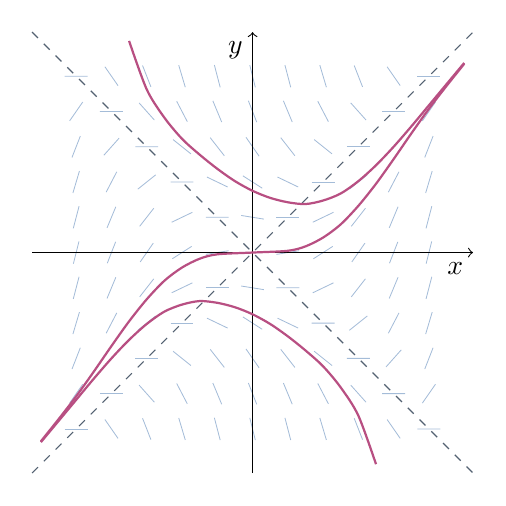
\begin{tikzpicture}[scale=1.12]
  \clip (-2.55,-2.55) rectangle (2.55,2.55);
  \foreach \xx in {-2,-1.6,...,2}{
    \foreach \yy in {-2,-1.6,...,2}{
      \pgfmathsetmacro{\ang}{atan(\xx*\xx-\yy*\yy)}
      \begin{scope}[shift={(\xx,\yy)},rotate=\ang]
        \draw[blue!45,line width=.3pt] (-.13,0)--(.13,0);
      \end{scope}
    }
  }
  \draw[gray,dashed] (-2.5,-2.5)--(2.5,2.5);
  \draw[gray,dashed] (-2.5,2.5)--(2.5,-2.5);
  \draw[->] (-2.5,0)--(2.5,0) node[below left] {$x$};
  \draw[->] (0,-2.5)--(0,2.5) node[below left] {$y$};
  \draw[pink,thick] plot[smooth] coordinates {(-1.4,2.40) (-1.2,1.85) (-1,1.53) (-.8,1.29) (-.6,1.11) (-.4,.95) (-.2,.81) (0,.70) (.2,.62) (.4,.57) (.6,.55) (.8,.59) (1,.67) (1.2,.81) (1.4,.99) (1.6,1.20) (1.8,1.43) (2,1.67) (2.2,1.91) (2.4,2.15)};
  \draw[pink,thick] plot[smooth] coordinates {(-2.4,-2.14) (-2.2,-1.89) (-2,-1.63) (-1.8,-1.35) (-1.6,-1.06) (-1.4,-.78) (-1.2,-.53) (-1,-.32) (-.8,-.17) (-.6,-.07) (-.4,-.02) (0,0) (.4,.02) (.6,.07) (.8,.17) (1,.32) (1.2,.53) (1.4,.78) (1.6,1.06) (1.8,1.35) (2,1.63) (2.2,1.89) (2.4,2.14)};
  \draw[pink,thick] plot[smooth] coordinates {(-2.4,-2.15) (-2.2,-1.91) (-2,-1.67) (-1.8,-1.43) (-1.6,-1.20) (-1.4,-.99) (-1.2,-.81) (-1,-.67) (-.8,-.59) (-.6,-.55) (-.4,-.57) (-.2,-.62) (0,-.70) (.2,-.81) (.4,-.95) (.6,-1.11) (.8,-1.29) (1,-1.53) (1.2,-1.85) (1.4,-2.40)};
\end{tikzpicture}
\par\small 图中蓝色短线表示方向场，粉色曲线是经过 $(0,0)$、$(0,\pm0.7)$ 的数值描画示例；灰色虚线是零斜率线。
\end{center}
\end{solution}

\begin{problem}{2.1-3}
试用欧拉折线法，取步长 $h=0.1$，求初值问题
  \[
  \begin{cases}
    \displaystyle \frac{dy}{dx}=x^2+y^2,\\
    y(1)=1
  \end{cases}
  \]
  的解在 $x=1.4$ 时的近似值。
\end{problem}

\begin{solution}
欧拉折线法使用递推式
\[
x_n=1+0.1n,\qquad y_{n+1}=y_n+0.1(x_n^2+y_n^2),\qquad y_0=1.
\]
逐步计算如下：
\[
\begin{array}{c|c|c|c}
n&x_n&y_n&x_n^2+y_n^2\\\hline
0&1.0&1.000000000&2.000000000\\
1&1.1&1.200000000&2.650000000\\
2&1.2&1.465000000&3.586225000\\
3&1.3&1.823622500&5.015599023
\end{array}
\]
故 $y_4=1.8236225+0.1\times5.015599023=2.325182402$，从而
\[\boxed{y(1.4)\approx2.3252}.\]
这是步长为 $0.1$ 的欧拉近似值，而非精确解的取值。
\note{配套参考书的提示写作约 $2.327$；按题定步长将四次欧拉递推逐项计算，得到上面的 $2.3252$。}
\end{solution}

\sect{2.2}
\begin{problem}{2.2-1}
试判断方程
  \[
    \frac{dy}{dx}=x\tan y
  \]
  在区域
  \[
    (1)\quad R_1:\ -1\le x\le1,\quad 0\le y\le\pi;
  \]
  \[
    (2)\quad R_2:\ -1\le x\le1,\quad -\frac{\pi}{4}\le y\le\frac{\pi}{4}
  \]
  上是否满足定理 2.2 的条件。
\end{problem}

\begin{solution}
定理 2.2 要求右端 $f(x,y)$ 在所考察区域连续，并对 $y$ 满足利普希茨条件。
在 $R_1$ 中包含 $y=\pi/2$，而 $\tan y$ 在这里无定义，所以条件不成立。
在 $R_2$ 中，$f(x,y)=x\tan y$ 与 $f_y=x\sec^2y$ 连续，并且
\[
|f_y|\le |x|\sec^2(\pi/4)\le2.
\]
由中值定理，$|f(x,y_1)-f(x,y_2)|\le2|y_1-y_2|$，故 $R_2$ 满足条件。
\end{solution}

\begin{problem}{2.2-2}
判断下列方程在什么样的区域上保证初值解存在且唯一：
  \begin{enumerate}[label=(\arabic*)]
    \item $y'=x^2+y^2$；
    \item $y'=x+\sin y$；
    \item $y'=x^{-1/3}$；
    \item $y'=\sqrt{|y|}$。
  \end{enumerate}
\end{problem}

\begin{solution}
在所说区域的每一点附近，检查右端是否连续以及是否对 $y$ 局部利普希茨：
\begin{enumerate}[label=(\arabic*)]
\item $f=x^2+y^2$ 与 $f_y=2y$ 在整个平面连续，故平面内任一点的初值解局部存在且唯一。
\item $f=x+\sin y$ 在整个平面连续，且 $|f_y|=|\cos y|\le1$，结论同上。
\item $f=x^{-1/3}$ 只在 $x\ne0$ 有定义。因此保证初值解存在且唯一的区域可取左半平面 $x<0$ 或右半平面 $x>0$；不能把 $x=0$ 纳入原方程的定义域。
\item $f=\sqrt{|y|}$ 在整个平面连续，所以处处有局部解；在 $y\ne0$ 的上、下半平面上，$f_y$ 局部有界，因而保证唯一性。在 $y=0$ 附近不能使用该唯一性定理，事实上零解可与离开横轴的解拼接，唯一性确实失败。
\end{enumerate}
\end{solution}

\begin{problem}{2.2-3}
讨论方程
  \[
    \frac{dy}{dx}=\frac{3}{2}y^{1/3}
  \]
  在什么样的区域中满足定理 2.2 的条件，并求通过 $(0,0)$ 的一切解。
\end{problem}

\begin{solution}
右端 $f(y)=\tfrac32y^{1/3}$ 处处连续，但在 $y=0$ 附近不满足对 $y$ 的利普希茨条件；在不与 $y=0$ 相交的区域上，$f_y=\tfrac12y^{-2/3}$ 局部有界，定理 2.2 适用。

先保留零解 $y\equiv0$。在 $y\ne0$ 的区间上分离变量，积分得
\[
\frac32y^{2/3}=\frac32(x-c),\qquad
y=\pm(x-c)^{3/2},\quad x\ge c.
\]
这里 $y^{2/3}=|y|^{2/3}$，因此非零支只能位于 $x\ge c$。若解通过 $(0,0)$，它可以在任意 $c\ge0$ 之前沿横轴停留，然后从 $c$ 向右选取正支或负支：
\[
\boxed{y(x)=\begin{cases}0,&x\le c,\\
\phantom{-}(x-c)^{3/2},&x\ge c,
\end{cases}\quad\text{或}\quad
y(x)=\begin{cases}0,&x\le c,\\
-(x-c)^{3/2},&x\ge c,
\end{cases}\qquad c\ge0.}
\]
两段在 $x=c$ 处的值和一阶导数都是零，代回原方程成立；再加上 $y\equiv0$，便得到全部解。
\end{solution}

\begin{problem}{2.2-4}
试用逐次逼近法求方程
  \[
    \frac{dy}{dx}=x-y^2
  \]
  满足初值条件 $y(0)=0$ 的近似解
  \[
    \varphi_0(x),\ \varphi_1(x),\ \varphi_2(x),\ \varphi_3(x).
  \]
\end{problem}

\begin{solution}
按皮卡迭代，取 $\varphi_0(x)=0$，并令
\[
\varphi_{n+1}(x)=\int_0^x\bigl(s-\varphi_n(s)^2\bigr)\,ds.
\]
于是
\[
\begin{aligned}
\varphi_0(x)&=0,\\
\varphi_1(x)&=\frac{x^2}{2},\\
\varphi_2(x)&=\int_0^x\left(s-\frac{s^4}{4}\right)ds
=\frac{x^2}{2}-\frac{x^5}{20},\\
\varphi_3(x)&=\int_0^x\left[s-\left(\frac{s^2}{2}-\frac{s^5}{20}\right)^2\right]ds\\
&=\boxed{\frac{x^2}{2}-\frac{x^5}{20}+\frac{x^8}{160}-\frac{x^{11}}{4400}}.
\end{aligned}
\]
特别要注意，平方中的交叉项为负，所以积分后的 $x^8$ 项为正。
\end{solution}

\begin{problem}{2.2-5}
利用逐次逼近法求方程
  \[
    \frac{dy}{dx}=y^2-x^2
  \]
  适合初值条件 $y(0)=1$ 的近似解
  \[
    \varphi_0(x),\ \varphi_1(x),\ \varphi_2(x).
  \]
\end{problem}

\begin{solution}
初值为 $y(0)=1$，故迭代从 $\varphi_0(x)=1$ 开始：
\[
\varphi_{n+1}(x)=1+\int_0^x\bigl(\varphi_n(s)^2-s^2\bigr)\,ds.
\]
由此算出
\[
\begin{aligned}
\varphi_0(x)&=1,\\
\varphi_1(x)&=1+\int_0^x(1-s^2)ds
=1+x-\frac{x^3}{3},\\
\varphi_2(x)&=1+\int_0^x\left[\left(1+s-\frac{s^3}{3}\right)^2-s^2\right]ds\\
&=\boxed{1+x+x^2-\frac{x^4}{6}-\frac{2x^5}{15}+\frac{x^7}{63}}.
\end{aligned}
\]
\note{配套参考书的提示把 $\varphi_0$ 印为 $0$，但本题初值为 $y(0)=1$，所以迭代起点必须取 $\varphi_0\equiv1$。}
\end{solution}

\begin{problem}{2.2-6}
试证明定理 2.2 中的 $n$ 次近似解 $\varphi_n(x)$ 与精确解 $\varphi(x)$ 有如下的误差估计式：
  \[
    |\varphi_n(x)-\varphi(x)|
    \le \frac{MN^n}{(n+1)!}|x-x_0|^{n+1}.
  \]
\end{problem}

\begin{solution}
记 $e_n(x)=|\varphi(x)-\varphi_n(x)|$。定理证明中在所用矩形上有 $|f|\le M$、对 $y$ 的利普希茨常数为 $N$，且 $\varphi_0\equiv y_0$。于是
\[
e_0(x)=\left|\int_{x_0}^x f(s,\varphi(s))\,ds\right|\le M|x-x_0|.
\]
若 $e_n(x)\le MN^n|x-x_0|^{n+1}/(n+1)!$，利用精确解和迭代解的积分方程，在 $x\ge x_0$ 时有
\[
\begin{aligned}
e_{n+1}(x)&\le N\int_{x_0}^x e_n(s)\,ds\\
&\le\frac{MN^{n+1}}{(n+1)!}\int_{x_0}^x(s-x_0)^{n+1}ds
=\frac{MN^{n+1}}{(n+2)!}(x-x_0)^{n+2}.
\end{aligned}
\]
$x\le x_0$ 时将积分方向反过来，计算相同。归纳即得题中的估计。
\end{solution}

\begin{problem}{2.2-7}
求初值问题
  \[
  \begin{cases}
    \displaystyle \frac{dy}{dx}=x+y+1,\\
    y(0)=0
  \end{cases}
  \]
  的皮卡逐次逼近序列，并通过求逼近序列的极限求出初值问题的解。
\end{problem}

\begin{solution}
取 $\varphi_0=0$，由积分方程得到
\[
\varphi_{n+1}(x)=\int_0^x\bigl(s+\varphi_n(s)+1\bigr)\,ds.
\]
前几项为 $\varphi_1=x+x^2/2$、$\varphi_2=x+x^2+x^3/6$。归纳可得对 $n\ge1$，
\[
\boxed{\varphi_n(x)=x+2\sum_{k=2}^{n}\frac{x^k}{k!}+\frac{x^{n+1}}{(n+1)!}}.
\]
确实，把此式代入递推积分式，常数项和各次幂的系数恰好给出 $n+1$ 的公式。在任意有界区间上，末项趋于零而指数级数收敛，故
\[
\varphi(x)=x+2\sum_{k=2}^{\infty}\frac{x^k}{k!}
=\boxed{2e^x-x-2}.
\]
直接求导可核对 $\varphi'=\varphi+x+1$ 且 $\varphi(0)=0$。
\end{solution}

\begin{problem}{2.2-8}
在条形区域 $a\le x\le b,\ |y|<+\infty$ 上，假设方程 (2.1) 的所有解都唯一，对其中任意两个解 $y_1(x),y_2(x)$，如果有 $y_1(x_0)<y_2(x_0)$，则必有
  \[
    y_1(x)<y_2(x),\qquad x_0\le x\le b.
  \]
\end{problem}

\begin{solution}
若结论不成立，则连续函数 $d(x)=y_2(x)-y_1(x)$ 满足 $d(x_0)>0$，却在某个 $x_1\in(x_0,b]$ 有 $d(x_1)\le0$。由介值定理，存在 $c\in(x_0,x_1]$ 使 $y_1(c)=y_2(c)$。两条曲线在 $c$ 给出了同一初值问题的解；按题设的唯一性，它们在共同定义区间上相同，特别在 $x_0$ 相同，矛盾。因此 $y_1(x)<y_2(x)$ 在 $[x_0,b]$ 上成立。
\end{solution}

\begin{problem}{2.2-9}
设 $y(x),g(x)$ 为 $[a,b]$ 上的非负连续函数，$f(x)\ge0$ 在 $[a,b]$ 上可积。若
  \[
    y(x)\le g(x)+\int_a^x f(s)y(s)\,ds,\qquad x\in[a,b],
  \]
  则
  \[
    y(x)\le g(x)+\int_a^x f(s)g(s)
    \exp\!\left[\int_s^x f(\tau)\,d\tau\right]ds,\qquad x\in[a,b].
  \]
  进而，若 $g(x)$ 还是单调非减函数，则有
  \[
    y(x)\le g(x)\exp\!\left[\int_a^x f(s)\,ds\right],\qquad x\in[a,b].
  \]
\end{problem}

\begin{solution}
令 $R(x)=\int_a^x f(s)y(s)\,ds$，则 $R(a)=0$，且由于 $f\ge0$，
\[
R'(x)=f(x)y(x)\le f(x)g(x)+f(x)R(x)
\]
几乎处处成立。记 $F(x)=\int_a^x f(s)ds$，乘以积分因子 $e^{-F(x)}$，得到
\[
\bigl(e^{-F(x)}R(x)\bigr)'\le e^{-F(x)}f(x)g(x).
\]
从 $a$ 积分到 $x$，再代回 $y(x)\le g(x)+R(x)$，即得
\[
\boxed{y(x)\le g(x)+\int_a^x f(s)g(s)
e^{\int_s^x f(\tau)d\tau}\,ds}.
\]
若 $g$ 非减，则对 $s\le x$ 有 $g(s)\le g(x)$。因此右侧不超过
\[
g(x)\left[1+\int_a^x f(s)e^{F(x)-F(s)}ds\right]
=g(x)e^{F(x)},
\]
其中最后一步利用 $(e^{F(x)-F(s)})'_{s}=-f(s)e^{F(x)-F(s)}$。这便是第二个结论。
\end{solution}

\sect{2.3}
\begin{problem}{2.3-1}
试证明：对任意的 $x_0$ 及满足条件 $0<y_0<1$ 的 $y_0$，方程
  \[
    \frac{dy}{dx}=\frac{y(y-1)}{1+x^2+y^2}
  \]
  的满足条件 $y(x_0)=y_0$ 的解 $y=y(x)$ 在 $(-\infty,+\infty)$ 内存在。
\end{problem}

\begin{solution}
右端 $f(x,y)=y(y-1)/(1+x^2+y^2)$ 在整个平面连续可微，因此局部解唯一。常值函数 $y=0$ 和 $y=1$ 都是解。初值位于两者之间，由唯一性，积分曲线不能穿过这两条常值解，故在其存在区间内始终有 $0<y(x)<1$。

若最大存在区间有有限端点 $\beta$，则当 $x\to\beta$ 时 $(x,y(x))$ 留在有界闭集内，且 $f$ 有界；因而 $y(x)$ 有有限极限。以 $(\beta,\lim y)$ 为初值可把解接续到 $\beta$ 之外，与最大性矛盾。左端同理，所以最大存在区间是 $\boxed{(-\infty,+\infty)}$。
\end{solution}

\begin{problem}{2.3-2}
指出方程
  \[
    \frac{dy}{dx}=(1-y^2)e^{xy^2}
  \]
  的每一个解的最大存在区间，以及当 $x$ 趋于这个区间的右端点时解的性状。
\end{problem}

\begin{solution}
右端 $F(x,y)=(1-y^2)e^{xy^2}$ 在平面上光滑，故每个初值有唯一的最大解。两条常值解 $y\equiv\pm1$ 把平面分为三个不相交的水平带；其他解不能跨越它们。

设 $y(x_0)=y_0$。分情形讨论：
\begin{enumerate}[label=(\arabic*)]
\item $-1<y_0<1$：解单调上升且始终夹在 $-1$ 与 $1$ 之间，故向左右都能延拓，最大区间为 $\mathbb R$。在 $x\ge\max\{x_0,0\}$ 上有 $e^{xy^2}\ge1$；若右端极限小于 $1$，导数便最终有正的下界，矛盾。因此 $\lim_{x\to+\infty}y(x)=1$。
\item $y_0=\pm1$：解分别恒为 $\pm1$，最大区间均为 $\mathbb R$。
\item $y_0>1$：解单调下降，向右被 $1$ 与 $y_0$ 夹住，故右端点为 $+\infty$，并由同样的下界论证得到 $\lim_{x\to+\infty}y(x)=1$。向左解增大；最大区间形如 $(\alpha,+\infty)$。若 $\alpha$ 有限，则必有 $\lim_{x\downarrow\alpha}y(x)=+\infty$。有限的 $\alpha$ 不可能小于 $0$：在任意 $x\le-\eta<0$ 的有界区间内，$(y^2-1)e^{xy^2}$ 对 $y\ge1$ 有统一上界，不会在有限时间爆破。因此 $\alpha\ge0$；若向左走到 $x=0$ 时 $y$ 仍有限，则可继续延拓至 $-\infty$，即 $\alpha=-\infty$。两种情形确会出现：在 $x_0=1$ 处取 $y_0=2$，由 $x\ge0$ 时 $-y'\ge y^2-1$ 可知向左至多经过 $\int_2^{\infty}(u^2-1)^{-1}du=\tfrac12\ln3<1$ 就会爆破；而取 $y_0>1$ 足够接近 $1$ 时，连续依赖性保证解可以到达 $x=0$。一般没有确定 $\alpha$ 的初等公式。
\item $y_0<-1$：解单调下降，向左被 $-1$ 与 $y_0$ 夹住，所以左端点为 $-\infty$。向右越过 $x=0$ 后，$y'=-(y^2-1)e^{xy^2}\le-(y^2-1)$；比较方程 $z'=-(z^2-1)$ 的负支在有限时间趋于 $-\infty$，可知本解的右端点 $\beta<+\infty$，且 $\lim_{x\uparrow\beta}y(x)=-\infty$。最大区间为 $(-\infty,\beta)$。
\end{enumerate}
这里“有限端点必趋于无穷”来自延拓定理：若 $x$ 与 $y$ 都保持有限，光滑右端允许继续延拓。
\note{配套参考书提示把 $y_0>1$ 的情形一概写为整个实轴。上面 $x_0=1,\ y_0=2$ 的比较计算表明，该说法对左端点并不总成立。}
\end{solution}

\begin{problem}{2.3-3}
设 $f(x,y)$ 在整个平面上连续有界，对 $y$ 有连续偏导数，试证明方程
  \[
    \frac{dy}{dx}=f(x,y)
  \]
  的任一解 $y=\varphi(x)$ 在区间 $(-\infty,+\infty)$ 内有定义。
\end{problem}

\begin{solution}
设 $|f(x,y)|\le M$。任取一个局部解及其初值 $(x_0,y_0)$，在其存在区间内有
\[
|y(x)-y_0|=\left|\int_{x_0}^{x}f(s,y(s))\,ds\right|\le M|x-x_0|.
\]
若最大区间有有限端点 $\beta$，则 $y$ 在靠近 $\beta$ 时有界，而且由上式在两点间的版本 $|y(x)-y(t)|\le M|x-t|$ 可知 $y(x)$ 有有限极限。$f$ 的连续性保证在该极限点还能解初值问题并延拓；$f_y$ 连续又保证局部唯一。这与最大区间矛盾。左端同理，故任一解均定义在 $\boxed{\mathbb R}$ 上。
\end{solution}

\begin{problem}{2.3-4}
讨论方程
  \[
    \frac{dy}{dx}=\frac{y^2-1}{2}
  \]
  的通过点 $(0,0)$ 的解，以及通过点 $(\ln2,-3)$ 的解的存在区间。
\end{problem}

\begin{solution}
先分离变量。除两条常值解 $y=\pm1$ 外，
\[
\frac{2\,dy}{y^2-1}=dx
\quad\Longrightarrow\quad
\ln\left|\frac{y-1}{y+1}\right|=x+C.
\]
在 $(0,0)$ 处，$\frac{y-1}{y+1}=-1$，所以
\[
\boxed{y(x)=\frac{1-e^x}{1+e^x}},\qquad x\in\mathbb R.
\]
在 $(\ln2,-3)$ 处，比例为 $2$，从而 $\frac{y-1}{y+1}=e^x$，即
\[
\boxed{y(x)=\frac{1+e^x}{1-e^x}},\qquad x\in(0,+\infty).
\]
后一式在 $x\downarrow0$ 时趋于 $-\infty$，因此不能向左越过 $0$；向右始终有定义。
\end{solution}

\begin{problem}{2.3-5}
在方程
  \[
    \frac{dy}{dx}=f(y)
  \]
  中，如果 $f(y)$ 在 $(-\infty,+\infty)$ 内连续可微，且
  \[
    yf(y)<0\qquad (y\ne0),
  \]
  求证方程满足 $y(x_0)=y_0$ 的解 $y(x)$ 在区间 $[x_0,+\infty)$ 上存在，且有
  \[
    \lim_{x\to+\infty}y(x)=0.
  \]
\end{problem}

\begin{solution}
由 $f$ 的连续性和 $yf(y)<0$ 可知 $f(0)=0$。因此 $y=0$ 是解，且因 $f$ 连续可微而满足局部唯一性。

若 $y_0>0$，则在 $y>0$ 时 $y'=f(y)<0$，解向右单调下降；它既不能穿过零解，也不会超过 $y_0$，所以留在 $[0,y_0]$ 内并可延拓至任意 $x\ge x_0$。其极限 $\ell\ge0$ 存在。若 $\ell>0$，连续性给出 $f(y(x))\to f(\ell)<0$，于是解最终以负的固定速度下降，与收敛到 $\ell$ 矛盾；故 $\ell=0$。$y_0<0$ 时解单调上升并留在 $[y_0,0]$，论证相同。$y_0=0$ 时是零解。综上，最大解在 $[x_0,+\infty)$ 上存在且 $\boxed{\lim_{x\to+\infty}y(x)=0}$。
\end{solution}

\begin{problem}{2.3-6}
设 $f(x),\varphi'(y)$ 在 $(-\infty,+\infty)$ 内连续且 $\varphi(\pm1)=0$，则对任意的 $x_0$ 和 $|y_0|\le1$，方程
  \[
    \frac{dy}{dx}=f(x)\varphi(y)
  \]
  满足 $y(x_0)=y_0$ 的解 $y(x)$ 的存在区间为 $(-\infty,+\infty)$。
\end{problem}

\begin{solution}
$\varphi'$ 连续说明 $\varphi$ 连续可微；$f(x)\varphi(y)$ 在任意有限矩形内对 $y$ 局部利普希茨。由 $\varphi(\pm1)=0$，$y=1$ 与 $y=-1$ 都是解。若 $|y_0|<1$，唯一性使所求解不能与两条边界解相交，因此 $|y(x)|<1$；若 $y_0=\pm1$，所求解就是对应的常值解。解始终被限制在 $[-1,1]$，在任意有限 $x$ 区间上右端连续有界，故两端都可继续延拓。最大存在区间为 $\boxed{(-\infty,+\infty)}$。
\end{solution}

\begin{problem}{2.3-7}
设 $f(x,y)$ 在 $(\alpha,\beta)\times(-\infty,+\infty)$ 上连续，$a(x)$ 和 $b(x)$ 在 $(\alpha,\beta)$ 上非负连续，且满足
  \[
    |f(x,y)|\le a(x)|y|+b(x),
  \]
  则
  \[
    \frac{dy}{dx}=f(x,y)
  \]
  的任一解的最大存在区间均为 $(\alpha,\beta)$。
\end{problem}

\begin{solution}
右端连续，先由局部存在定理取任一解。固定包含初值 $x_0$ 的紧区间 $[u,v]\subset(\alpha,\beta)$，并令 $A=\max_{[u,v]}a$、$B=\max_{[u,v]}b$。积分方程给出对 $x\ge x_0$，
\[
|y(x)|\le |y_0|+B(x-x_0)+A\int_{x_0}^x|y(s)|\,ds.
\]
应用本章的贝尔曼不等式，得到 $|y(x)|\le(|y_0|+B(v-u))e^{A(v-u)}$；向左积分也有相同类型的界。因此解在任何有限的内点区间都不会趋于无穷。若最大存在区间在 $(\alpha,\beta)$ 内有有限端点，连续右端及上述界使解有有限极限，可在该点继续求解，矛盾。故每个最大解的存在区间恰为 $\boxed{(\alpha,\beta)}$。这里无需额外假设唯一性。
\end{solution}

\sect{2.4}
\begin{problem}{2.4-1}
判断下列方程是否有奇解？如果有奇解，求出奇解，并作图。
  \begin{enumerate}[label=(\arabic*)]
    \item $\displaystyle \frac{dy}{dx}=\sqrt{|y|}$；
    \item $\displaystyle \frac{dy}{dx}=\sqrt{y-x}$；
    \item $\displaystyle \frac{dy}{dx}=-x\pm\sqrt{x^2+2y}$。
  \end{enumerate}
\end{problem}

\begin{solution}
本节称一条本身也是方程解、且与一族其他积分曲线相切的曲线为奇解。逐项检查边界曲线是否满足原方程：
\begin{enumerate}[label=(\arabic*)]
\item 在 $y\ne0$ 上分离变量。正支为 $y=(x-c)^2/4$，取 $x\ge c$；负支为 $y=-(x-c)^2/4$，取 $x\le c$。两者都在 $(c,0)$ 与横轴相切。$\boxed{y=0}$ 本身也是解，且可与这些非零支作可微拼接，故是奇解。图像为横轴及其上下两侧与横轴相切的抛物线弧。
\item 方程只在 $y\ge x$ 有意义。若候选边界 $y=x$ 是解，它须满足 $y'=1$；但代入右端得 $\sqrt{y-x}=0$，两边不等。因此 $y=x$ 不是解，也就不是奇解。事实上令 $z=\sqrt{y-x}>0$，可得 $1+2zz'=z$，可继续描画区域内的曲线，但它们不会产生一条边界奇解。
\item 令 $z=\sqrt{x^2+2y}\ge0$。在 $z>0$ 处由 $2zz'=2x+2y'$ 得 $z'=1$（正号方程）或 $z'=-1$（负号方程）。所以普通积分曲线是直线族 $y=-cx+c^2/2$ 的适当半支；当 $x=c$ 时，它们与抛物线 $\boxed{y=-x^2/2}$ 相切。该抛物线的导数为 $-x$，而右端在 $x^2+2y=0$ 上也为 $-x$，因此它确为两个符号方程的奇解。图像为这条开口向下的抛物线及其切线族。
\end{enumerate}
\begin{center}
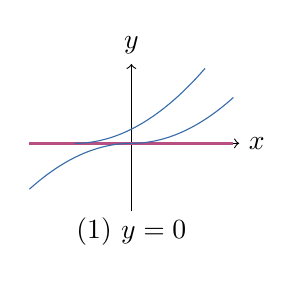
\begin{tikzpicture}[scale=.72]
  \draw[->] (-1.8,0)--(1.9,0) node[right]{$x$};
  \draw[->] (0,-1.2)--(0,1.4) node[above]{$y$};
  \draw[pink,very thick] (-1.8,0)--(1.8,0);
  \draw[blue,domain=-1:1.3,samples=40] plot (\x,{(\x+1)^2/4});
  \draw[blue,domain=0:1.8,samples=40] plot (\x,{\x*\x/4});
  \draw[blue,domain=-1.8:0,samples=40] plot (\x,{-\x*\x/4});
  \node at (0,-1.55) {(1) $y=0$};
\end{tikzpicture}\hspace{1em}
\begin{tikzpicture}[scale=.72]
  \draw[->] (-1.8,0)--(1.9,0) node[right]{$x$};
  \draw[->] (0,-1.2)--(0,1.4) node[above]{$y$};
  \draw[pink,dashed,thick] (-1.1,-1.1)--(1.25,1.25);
  \draw[blue,thick] (-1.8,-.8)--(.4,1.4);
  \node at (0,-1.55) {(2) $y=x$ 非解};
\end{tikzpicture}\hspace{1em}
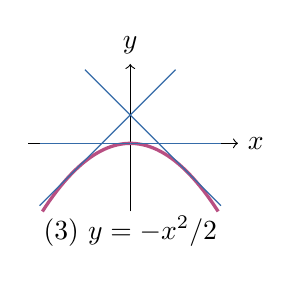
\begin{tikzpicture}[scale=.72]
  \draw[->] (-1.8,0)--(1.9,0) node[right]{$x$};
  \draw[->] (0,-1.2)--(0,1.4) node[above]{$y$};
  \draw[pink,very thick,domain=-1.55:1.55,samples=50] plot (\x,{-\x*\x/2});
  \draw[blue] (-1.6,-1.1)--(.8,1.3);
  \draw[blue] (-.8,1.3)--(1.6,-1.1);
  \draw[blue] (-1.6,0)--(1.6,0);
  \node at (0,-1.55) {(3) $y=-x^2/2$};
\end{tikzpicture}
\par\small 粉色实线为奇解；第二幅的粉色虚线仅为定义域边界，不是解。蓝线表示普通解的示意。
\end{center}
\end{solution}

\begin{problem}{2.4-2}
求一曲线，具有如下性质：曲线上任一点的切线，在 $x,y$ 轴上的截距之和为 $1$。
\end{problem}

\begin{solution}
设所求曲线在某点的切线斜率为 $p=y'$，写为 $Y=pX+b$。它在两轴上的有向截距分别为 $-b/p$、$b$，故题意给出 $b-b/p=1$，即 $b=p/(p-1)$。于是切线条件化为 Clairaut 方程
\[
y=xp+\frac{p}{p-1},\qquad p=y',\quad p\ne0,1.
\]
对 $x$ 求导并消去两边的 $p$，得 $\bigl(x-(p-1)^{-2}\bigr)p'=0$。一类解是直线族
\[
y=Cx+\frac{C}{C-1},\qquad C\ne0,1.
\]
若要寻找以这些直线为切线的一条非直线曲线，则取另一支 $x=(p-1)^{-2}$，代回得
\[
\boxed{x=\frac1{(p-1)^2},\qquad y=\frac{p^2}{(p-1)^2}\quad(p\ne0,1).}
\]
这是所求包络线的参数形式。消去 $p$ 可写成 $y=(1\pm\sqrt{x})^2$ 的相应弧段；每个参数值的切线截距和都为 $1$。
\end{solution}

\begin{problem}{2.4-3}
求一曲线，此曲线的任一切线在两个坐标轴间的线段长等于 $a$。
\end{problem}

\begin{solution}
设切线与两轴的交点为 $(A,0)$、$(0,B)$，则 $A^2+B^2=a^2$。令 $A=a\cos t$、$B=a\sin t$，在两个截距非零的弧段上，切线族写成
\[
\frac{x}{a\cos t}+\frac{y}{a\sin t}=1.
\]
包络线上的点既满足此式，也满足对参数 $t$ 求导后得到的式子。联立解出 $x=a\cos^3t$、$y=a\sin^3t$。因此所求曲线为
\[
\boxed{x=a\cos^3t,\qquad y=a\sin^3t,}
\]
消去参数即 $\boxed{|x|^{2/3}+|y|^{2/3}=a^{2/3}}$。反过来，此参数曲线的切线截距为 $a\cos t$、$a\sin t$，两截距间的距离确为 $a$。
\note{严格讨论“两轴截距”时取 $\sin t\cos t\ne0$ 的光滑弧段；坐标轴上的尖点是这些弧段的极限点。}
\end{solution}

\begin{problem}{2.4-4}
应用 $p$--判别法求下列方程的奇解：
  \begin{enumerate}[label=(\arabic*)]
    \item $y=xy'+(y')^2$；
    \item $\displaystyle y=xy'+\frac{1}{y'}$；
    \item $\displaystyle (y-1)^2(y')^2=\frac49y$；
    \item $\displaystyle (y-1)^2(y')^2=ye^{xy}$。
  \end{enumerate}
\end{problem}

\begin{solution}
记 $p=y'$，把各方程写为 $F(x,y,p)=0$。$p$--判别曲线由 $F=F_p=0$ 求出，但候选曲线还必须代回原方程，并核对其与普通积分曲线相切。
\begin{enumerate}[label=(\arabic*)]
\item $F=y-xp-p^2$，$F_p=-x-2p$。故 $p=-x/2$，代回得 $\boxed{y=-x^2/4}$；其导数正是 $-x/2$。普通解 $y=Cx+C^2$ 与它在 $x=-2C$ 相切，所以它是奇解。
\item $F=y-xp-1/p$（$p\ne0$），$F_p=-x+1/p^2$。于是 $x=1/p^2$、$y=2/p$，消去 $p$ 得 $\boxed{y^2=4x}$。其两支满足 $p=2/y$，代回原方程成立；普通解 $y=Cx+1/C$（$C\ne0$）在 $x=1/C^2$ 与它相切。因此两支组成奇解曲线。
\item $F=(y-1)^2p^2-4y/9$，$F_p=2(y-1)^2p$。若 $y=1$，则 $F=-4/9\ne0$；若 $p=0$，则 $y=0$。所以唯一候选为 $\boxed{y=0}$。它满足原方程，且在 $y=0$ 处可与非零解的分支相切，因而是奇解。
\item $F=(y-1)^2p^2-ye^{xy}$，$F_p=2(y-1)^2p$。$y=1$ 不能使 $F=0$；$p=0$ 给出 $y=0$。故奇解为 $\boxed{y=0}$。在 $y$ 接近 $0$ 时，非零支的斜率为 $p=\pm\sqrt{ye^{xy}}/|y-1|$，趋于零，说明这些分支与零解相切。
\end{enumerate}
\end{solution}

\sect{2.5}
\begin{problem}{2.5-1}
试用贝尔曼不等式证明：若方程
  \[
    \frac{dy}{dx}=f(x,y)\tag{*}
  \]
  满足
  \begin{enumerate}[label=(\arabic*)]
    \item $f(x,y)$ 在区域 $D$ 内连续且满足利普希茨条件；
    \item $y=\varphi(x)$ 是方程 (*) 定义在 $a\le x\le b$ 上的解，且 $y_0=\varphi(x_0)$，
  \end{enumerate}
  则对于 $\varepsilon>0$，恒存在 $\delta(\varepsilon)>0$，使得对任何适合
  \[
    |R(x,y)|<\delta(\varepsilon)\qquad ((x,y)\in D)
  \]
  的连续函数 $R(x,y)$，方程
  \[
    \frac{dy}{dx}=f(x,y)+R(x,y)
  \]
  的满足条件 $y(x_0)=y_0$ 的解 $y=\widetilde{\varphi}(x)$ 在 $a\le x\le b$ 上有定义，且
  \[
    |\widetilde{\varphi}(x)-\varphi(x)|<\varepsilon.
  \]
\end{problem}

\begin{solution}
令 $L$ 为 $f$ 在 $D$ 内对 $y$ 的利普希茨常数，$T=b-a$。原解的轨迹
$K=\{(x,\varphi(x)):a\le x\le b\}$ 是 $D$ 内的紧集，可选 $\rho>0$，使其宽为 $\rho$ 的闭管状邻域仍包含于 $D$。取
\[
0<\delta(\varepsilon)<\frac{\min\{\rho,\varepsilon\}}{T e^{LT}}
\]
（$T=0$ 时命题显然）。连续的 $f+R$ 保证扰动初值问题至少有局部解。只要该解仍在上述邻域内，记 $e(x)=|\widetilde\varphi(x)-\varphi(x)|$，由两条积分方程及 $|R|<\delta$ 得
\[
e(x)\le L\left|\int_{x_0}^x e(s)\,ds\right|+\delta|x-x_0|.
\]
对 $x\ge x_0$ 用贝尔曼不等式（或对 $x\le x_0$ 反向积分）可得
\[
e(x)\le\delta|x-x_0|e^{L|x-x_0|}
\le\delta T e^{LT}<\min\{\rho,\varepsilon\}.
\]
因误差严格小于 $\rho$，解不可能先从管状邻域逃出；又因它在任意有限 $x$ 区间内保持有界，连续右端的延拓定理保证它可延至整个 $[a,b]$。上述估计随即给出 $\boxed{|\widetilde\varphi(x)-\varphi(x)|<\varepsilon}$。$R$ 只须连续，扰动解未必唯一，但每一个通过该初值的解都满足估计。
\end{solution}

\begin{problem}{2.5-2}
已知方程
  \[
    \frac{dy}{dx}=\sin(xy),
  \]
  试求
  \[
    \left.\frac{\partial y(x,x_0,y_0)}{\partial x_0}\right|_{x_0=0,\ y_0=0}
    \quad\text{和}\quad
    \left.\frac{\partial y(x,x_0,y_0)}{\partial y_0}\right|_{x_0=0,\ y_0=0}.
  \]
\end{problem}

\begin{solution}
在 $x_0=y_0=0$ 时，$y(x)\equiv0$ 是方程的解。对初值 $y_0$ 的偏导数 $u(x)=\partial y/\partial y_0$ 满足本节的变分方程
\[
u'=f_y(x,0)u=xu,\qquad u(0)=1,
\]
因为 $f(x,y)=\sin(xy)$ 的 $y$ 偏导数为 $f_y=x\cos(xy)$。积分得
\[
\boxed{\left.\frac{\partial y}{\partial y_0}\right|_{x_0=y_0=0}
=e^{x^2/2}}.
\]
改变起始时刻 $x_0$ 而仍令 $y_0=0$，零解始终不变，故
\[
\boxed{\left.\frac{\partial y}{\partial x_0}\right|_{x_0=y_0=0}=0}.
\]
\note{配套参考书的习题提示把第一个偏导数写为 $1$；变分方程显示它应为 $e^{x^2/2}$，只有 $x=0$ 时才等于 $1$。}
\end{solution}

\begin{problem}{2.5-3}
设 $\varphi(x,x_0,y_0)$ 是初值问题
  \[
  \begin{cases}
    \displaystyle \frac{dy}{dx}=f(x,y),\\
    y(x_0)=y_0
  \end{cases}
  \]
  的解，试证明
  \[
    \frac{\partial\varphi(x,x_0,y_0)}{\partial x_0}
    +
    \frac{\partial\varphi(x,x_0,y_0)}{\partial y_0}f(x_0,y_0)=0.
  \]
\end{problem}

\begin{solution}
固定 $(x_0,y_0)$，设 $Y(x)=\varphi(x,x_0,y_0)$。沿同一条解曲线，在稍后的起始时刻 $x_0+h$，初值应为
\[
Y(x_0+h)=y_0+h f(x_0,y_0)+o(h).
\]
解的唯一性给出流的拼接关系
\[
\varphi\bigl(x,x_0+h,Y(x_0+h)\bigr)
=\varphi(x,x_0,y_0).
\]
在本节保证解对初值可微的条件下，对 $h$ 在 $0$ 处求导，右端为常数，左端由链式法则得到
\[
\boxed{\frac{\partial\varphi}{\partial x_0}(x,x_0,y_0)
+f(x_0,y_0)\frac{\partial\varphi}{\partial y_0}(x,x_0,y_0)=0}.
\]
这个等式表示：沿同一解曲线平移起始时刻并相应调整初值，不会改变后来时刻的解值。
\end{solution}

\begin{problem}{2.5-4}
设 $p(x)$ 和 $q(x)$ 是连续函数，$\varphi(x,x_0,y_0)$ 是初值问题
  \[
    \frac{dy}{dx}+p(x)y=q(x),\qquad y(x_0)=y_0
  \]
  的解。求
  \[
    \frac{\partial\varphi(x,x_0,y_0)}{\partial x_0}
    \quad\text{和}\quad
    \frac{\partial\varphi(x,x_0,y_0)}{\partial y_0}.
  \]
\end{problem}

\begin{solution}
令 $P(s,t)=\int_s^t p(\tau)\,d\tau$。积分因子法给出
\[
\varphi(x,x_0,y_0)=e^{-P(x_0,x)}y_0
+\int_{x_0}^{x}e^{-P(s,x)}q(s)\,ds.
\]
因此对 $y_0$ 求导，直接得到
\[
\boxed{\frac{\partial\varphi}{\partial y_0}=e^{-\int_{x_0}^x p(s)\,ds}}.
\]
对 $x_0$ 求导时，第一项的导数为 $p(x_0)y_0e^{-P(x_0,x)}$，积分项按下限求导得到 $-q(x_0)e^{-P(x_0,x)}$，故
\[
\boxed{\frac{\partial\varphi}{\partial x_0}
=\bigl[p(x_0)y_0-q(x_0)\bigr]e^{-\int_{x_0}^x p(s)\,ds}}.
\]
因 $f(x_0,y_0)=q(x_0)-p(x_0)y_0$，两式也满足上题的关系。
\end{solution}

\begin{problem}{2.5-5}
在方程
  \[
    \frac{dy}{dx}=f(x,y)
  \]
  中，设 $f(x,y)$ 在区域 $D$ 内连续且满足利普希茨条件，$y=\varphi(x)$ 是该方程定义在 $[a,b]$ 上的解且 $y_0=\varphi(x_0)$。则对任意的 $\varepsilon>0$，存在 $\delta(\varepsilon)>0$，使得对任何满足
  \[
    |g(x,y)|<\delta(\varepsilon),\qquad x\in D
  \]
  的连续函数 $g(x,y)$，方程
  \[
    \frac{dy}{dx}=f(x,y)+g(x,y)
  \]
  的满足 $y(x_0)=y_0$ 的解 $\widetilde{\varphi}(x)$ 在 $[a,b]$ 上有定义且
  \[
    |\widetilde{\varphi}(x)-\varphi(x)|<\varepsilon.
  \]
\end{problem}

\begin{solution}
本题与第 1 题的断言相同，只是把扰动记为 $g$。为明确界的来源，仍设 $L$ 为 $f$ 对 $y$ 的利普希茨常数，$T=b-a$，并选取原解曲线周围宽 $\rho$、仍位于 $D$ 内的闭管状邻域。令
\[
0<\delta(\varepsilon)<\frac{\min\{\rho,\varepsilon\}}{T e^{LT}}.
\]
若 $|g|<\delta$，两解的积分方程相减，对任意位于管内的 $x$ 得
\[
|\widetilde\varphi(x)-\varphi(x)|
\le L\left|\int_{x_0}^x(\widetilde\varphi(s)-\varphi(s))\,ds\right|
+\delta|x-x_0|.
\]
贝尔曼不等式给出误差小于 $\delta T e^{LT}<\min\{\rho,\varepsilon\}$。因此扰动解不能先触及管的边界；连续右端保证局部存在，保持在管内又保证继续延拓到 $[a,b]$。从而在全区间内 $\boxed{|\widetilde\varphi-\varphi|<\varepsilon}$。
\end{solution}

\end{document}
